\section{Method}
\label{sec:method}
As visualized in \Cref{fig:pipeline}, our method consists of three major components: foveal-periphery image synthesis (\Cref{sec:method:net}), and real-time blending with optimized spatial-temporal precision (\Cref{sec:method:blending}).

%\subsection{Pipeline}
\begin{figure*}[htb]
    \centering
    \includegraphics[width=\linewidth]{TOG/figs/sys_pipeline.png}
    \Caption{System pipeline.}
    {%
    }
    \label{fig:pipeline}
\end{figure*}

%To meet the requirement of real-time, use fewer channels/layers, much fewer samples, predict a coarse fovea image, then refine using local view guidance

\subsection{GazeNet}
\label{sec:method:net}
\begin{figure*}[htb]
    \centering
    \includegraphics[width=\linewidth]{TOG/figs/spher_net_flow.png}
    \caption{GazeNet Network.}
    \label{fig:my_label}
\end{figure*}

%Follow NeRF's idea, represent scene using a MLP but in spherical space because we are inside-out (viewer is located at center area and look around)

\qisun{(Jan 9, 2021) Avoid usage of subsubsection.}
\paragraph{Multi spherical representation}
As reviewed in \autoref{sec:prior}, prior work contributed a lot to represent a static scene via object-focused manner. Inspired by that, we investigate on how to represent a static scene for VR environment to render real-timely without loading the entire scene. However, VR environment is user-centered. That is, unlike the object-focused ``outside-in'' way such as \cite{mildenhall2020nerf}, the views are highly varied in an ``inside-out'' fashion. 
Consequently, the overlaps among views are diversified, resulting in training challenges for large virtual scenes.
To address this problem, we depict a VR scene as concentric spherical volumes with the center as the original point, as visualized in \Cref{fig:teaser:scene}. 

%\begin{figure}[htb]
%    \centering
%    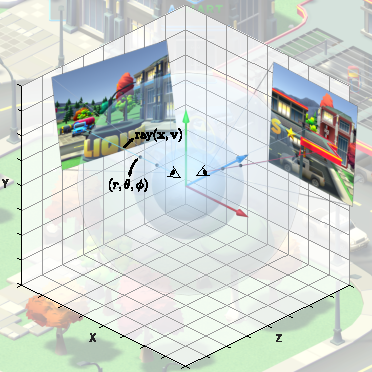
\includegraphics[width=0.96\linewidth]{TOG/figs/spher_coord.pdf}
%%    \caption{Visualization of our multi-spherical coordinate system.}
    \label{fig:method:coordinate}
%\end{figure}
% different position (10cm working, 50cm not working),
% different rotation

\dnc{(Jan 11) Ray to spherical coord} For a sphere with radius $r$, the intersection of ray and sphere $\pt_r$ can be calculated by solving:

\begin{equation}
    \|\pt_r\|^2=\|\rayo + k\rayd\|^2=r^2
\end{equation}

Convert $\pt_r$ to spherical coordinate $(r, \theta, \phi)$:

\begin{equation}
    \begin{cases}
        \theta = \mathrm{atan2}(x_{\pt_r}/z_{\pt_r})\\
        \phi = \mathrm{acos}(y_{\pt_r} / r)
    \end{cases}
\end{equation}

\dnc{(Jan 11) A simple derivation for the requirement of depth range and samples} Take 2D as an example. Consider two view centers $\rayo_1$, $\rayo_2$ on X axis and a point $\pt$ in 3D space. The radius of nearest sampling sphere of $\pt$ is $r_l$. The intersections of the sphere and rays from $\rayo_1$, $\rayo_2$ to $\pt$ are $\pt'_{1,r_l}$ and $\pt'_{2,r_l}$, respectively. $\Delta\pt'_{r_l}=\|\pt'_{2,r_l}-\pt'_{1,r_l}\|$ is small enough, then we have:

\begin{equation}
    \Delta\pt'_{r_l} \approx \Delta\rayo \frac{|z_\pt - r_l|}{z_\pt}
\end{equation}

\begin{equation}
    hello
\end{equation}

\begin{figure}[htb]
    \centering
    \includegraphics[width=0.96\linewidth]{TOG/figs/depth_disparity.pdf}
    \caption{Depth disparity}
    \label{fig:method:eccentricity}
\end{figure}

With this coordinate system, the input of individual element in the 3D spaces is defined as $p=(r, \theta, \phi)$ and the output is color information $c=(r,g,b)$ and volume density $d$. We train the scene representation with an multilayer perception (MLP) network first. 
For the training uniformity and run-time efficiency, we do not distinguish different eccentricities during the training stage. Instead, the spatially variant visual acuity is represented as varying field of views in the rendering, i.e., data creation.
Specifically, we depict the whole visual field as three semantic layers the fovea ({0-10 deg}), mid-periphery {6-60 deg}, and far periphery {y-110 deg}. In each frame, The uniformized networks returns three images with a identical resolution yet, as seen from the separation range in deg, gradually larger areas along eccentricity.

\begin{figure}[htb]
    \centering
    \includegraphics[width=0.96\linewidth]{TOG/figs/layers_together_zh.pdf}% try not overlapping the text on the image since we want the reviewers to see each pixel clearly
    \caption{Visualization of the output at three eccentricity ranges.}
    \label{fig:method:eccentricity}
\end{figure}

%estimate the fovea, mid-peripheral, peripheral field of view for a novel view next, fine-tune the fovea result with local view streamed from the cloud, and lastly warp/blend the three results for VR display.

\paragraph{Input encoding}
Since the input of our representation network is only three dimensional, we map the inputs to a higher dimensional space via high-frequency functions. \qisun{(Jan 9, 2021) What is bad if we have low-dim input? Harder to converge, higher error etc.?} \zh{(Jan 9) similar to NeRF, three components are not sufficient for achieving state-of-the-art quality, as demonstrated in Section 6.4). We introduce a positional encoding of the input coordinates that assists the MLP in
representing high-frequency functions.}
Thus we encoded the input through function:
\begin{align}
\iota (p) = (\sin(2^0 p), \cos(2^0 p), ..., \sin(2^{L-1}p, \cos(2^{L-1}p))
\label{eqn:inputencode}
\end{align}
The function $\iota (\cdot)$ is applied to each of the 3D location representation ($r$, $\theta$, and $\phi$), we choose $L$ to be 10 in practice. Hence, the input dimension becomes 3 x 20 = 60 after encoding. The MLP network is composed with $N_{layer}$ fully-connected layers, each uses ReLu as activation function and $N_{channel}$ channels per layer and output the color and volume density.

\paragraph{Synthesis}
% the description of the volume density is the same as chapter 4 in NeRF paper.
Similar to \cite{mildenhall2020nerf}, the trained representation is then deployed to synethesis final images via ray marching. For accelerating the performance, we bounded the near/far range to $20$ and $50$ meters respectively. The bounding, however, may introduce subtle quality drop, as shown in \Cref{fig:method:bounding}.
\begin{figure}
    \centering
    \subfloat[w bounding]{\includegraphics[width = 0.47\linewidth]{TOG/figs/depth_without_bound.png}}\hspace{1em}
    \subfloat[w/o bounding]{\includegraphics[width = 0.47\linewidth]{TOG/figs/depth_with_bound.png}}
    \caption{Visualization of ray marching bounding.}
    \label{fig:method:bounding}
\end{figure}
%For each pixel, we perform a ray from the camera and accumulate all the intersection's color weighted by the density accordingly between near bound and far bound. In practice, we experimented with different far bound values: 20 (meters) and 50 (meters), the difference between output is minimal. (\note{add figure for comparison}). We also experimented with the sampling number ($N_{sample}$) for accumulation between near bound and far bound to balance time cost and effects. Hence, we have an output image for the camera perspective.
However, as a gaze-contingent method, the compromised quality would be unnoticeable in periphery. Thus, we further refine the visual quality in foveal vision, as detailed in \Cref{sec:method:refine}.
Since we aim to render a novel view in real time and with perceptually high quality, we estimate the foveated image (10 degree), middle peripheral image (60 degree), and full peripheral image (110 degree) from the same novel view for further synthesis. Regarding foveated rendering, we estimate an image with size of 64 x 64, $N_{layer}=12$, $N_{channel}=64$, and $N_{sample}=16$. Regarding middle peripheral and full peripheral rendering, we estimate the two images with size of 256 x 256, $N_{layer}=8$, $N_{channel}=64$, and $N_{sample}=4$. We next upsample middle peripheral to ??? x ??? and full peripheral to 1440 x 1440 for blending.
\nothing{
\subsection{Refinement for Fovea Layer}
\label{sec:method:refine}
Due to the depth bounding and prediction errors, it is particularly challenging to preserve pixel-wise quality without compromising real-time performance. However, the human foveal vision is remarkably sensitive to subtle details across all frequency ranges. To 
To maximize the quality of foveated image, we utilize the limited but consistent network bandwidth by retrieving a local peripheral image from the cloud. The retrieval was realized by cloud-based rendering using users' upstreamed head and gaze parameters.
Due to the inevitable dual-way transmission, it is impossible to instantly obtain the image without latency. Displaying outdated frames have been studied as a major cause of simulator sickness.
}%nothing
\note{describe when to retrieve new full peripheral image.} We leverage local guidance views to fine tune the output foveated image. Local guidance view is decided according to current camera view. We chose the nearest 4 views (or 8 views) as reference views and estimate the color as well as volume density for all reference views. Every time we receive a new peripheral image from the cloud, we calculate the delta between the ground truth and our result for reference views for preparation. Then we warp the delta into target camera view, calculate the average and apply to the fovea result for each frame.

\subsection{Real-time Rendering}
% \subsection{Fovea-Peripheral Blending}
\label{sec:method:blending}
Lastly, we apply alpha blend on the fine-tuned fovea view and middle peripheral view, as well as on the middle peripheral view and full peripheral view via function smo/:

\subsection{Latency-quality joint optimization}
\label{sec:method:optimization}
Increasing rendering sampling naturally improves the image output quality. However, it increases the latency, causing quality drop stretched along time, and more critically, simulator sickness.
Inspired by \cite{Li:2020:TSP}, we perform a spatial-temporal joint optimization to determine the sampling that adapts to individual computational resources. This is achieved via a Pareto efficiency optimization. 

$E_{q}\triangleq $

$E_{l}$ is defined as the loss introduced by latency. 
\begin{align}
    \int E_{l} \mathbf{d} t
\end{align}

\begin{figure*}
    \centering
    \subfloat[quality-only]{\includegraphics[width=0.32\linewidth]{example-image-a}}
    \subfloat[latency-only]{\includegraphics[width=0.32\linewidth]{example-image-a}}
    \subfloat[ours]{\includegraphics[width=0.32\linewidth]{example-image-a}}
    \caption{Latency-quality joint-optimization.}
    \label{fig:optimization}
\end{figure*}

%\subsection{Cloud-Based System}
%\label{sec:method:system}
%Finally, we deploy our gaze-contingent synthesizer to a real-time cloud-based streaming system.